\pgfdeclareplotmark{cross} {
\pgfpathmoveto{\pgfpoint{-0.3\pgfplotmarksize}{\pgfplotmarksize}}
\pgfpathlineto{\pgfpoint{+0.3\pgfplotmarksize}{\pgfplotmarksize}}
\pgfpathlineto{\pgfpoint{+0.3\pgfplotmarksize}{0.3\pgfplotmarksize}}
\pgfpathlineto{\pgfpoint{+1\pgfplotmarksize}{0.3\pgfplotmarksize}}
\pgfpathlineto{\pgfpoint{+1\pgfplotmarksize}{-0.3\pgfplotmarksize}}
\pgfpathlineto{\pgfpoint{+0.3\pgfplotmarksize}{-0.3\pgfplotmarksize}}
\pgfpathlineto{\pgfpoint{+0.3\pgfplotmarksize}{-1.\pgfplotmarksize}}
\pgfpathlineto{\pgfpoint{-0.3\pgfplotmarksize}{-1.\pgfplotmarksize}}
\pgfpathlineto{\pgfpoint{-0.3\pgfplotmarksize}{-0.3\pgfplotmarksize}}
\pgfpathlineto{\pgfpoint{-1.\pgfplotmarksize}{-0.3\pgfplotmarksize}}
\pgfpathlineto{\pgfpoint{-1.\pgfplotmarksize}{0.3\pgfplotmarksize}}
\pgfpathlineto{\pgfpoint{-0.3\pgfplotmarksize}{0.3\pgfplotmarksize}}
\pgfpathclose
\pgfusepathqstroke
}
\pgfdeclareplotmark{cross*} {
\pgfpathmoveto{\pgfpoint{-0.3\pgfplotmarksize}{\pgfplotmarksize}}
\pgfpathlineto{\pgfpoint{+0.3\pgfplotmarksize}{\pgfplotmarksize}}
\pgfpathlineto{\pgfpoint{+0.3\pgfplotmarksize}{0.3\pgfplotmarksize}}
\pgfpathlineto{\pgfpoint{+1\pgfplotmarksize}{0.3\pgfplotmarksize}}
\pgfpathlineto{\pgfpoint{+1\pgfplotmarksize}{-0.3\pgfplotmarksize}}
\pgfpathlineto{\pgfpoint{+0.3\pgfplotmarksize}{-0.3\pgfplotmarksize}}
\pgfpathlineto{\pgfpoint{+0.3\pgfplotmarksize}{-1.\pgfplotmarksize}}
\pgfpathlineto{\pgfpoint{-0.3\pgfplotmarksize}{-1.\pgfplotmarksize}}
\pgfpathlineto{\pgfpoint{-0.3\pgfplotmarksize}{-0.3\pgfplotmarksize}}
\pgfpathlineto{\pgfpoint{-1.\pgfplotmarksize}{-0.3\pgfplotmarksize}}
\pgfpathlineto{\pgfpoint{-1.\pgfplotmarksize}{0.3\pgfplotmarksize}}
\pgfpathlineto{\pgfpoint{-0.3\pgfplotmarksize}{0.3\pgfplotmarksize}}
\pgfpathclose
\pgfusepathqfillstroke
}
\pgfdeclareplotmark{newstar} {
\pgfpathmoveto{\pgfqpoint{0pt}{\pgfplotmarksize}}
\pgfpathlineto{\pgfqpointpolar{44}{0.5\pgfplotmarksize}}
\pgfpathlineto{\pgfqpointpolar{18}{\pgfplotmarksize}}
\pgfpathlineto{\pgfqpointpolar{-20}{0.5\pgfplotmarksize}}
\pgfpathlineto{\pgfqpointpolar{-54}{\pgfplotmarksize}}
\pgfpathlineto{\pgfqpointpolar{-90}{0.5\pgfplotmarksize}}
\pgfpathlineto{\pgfqpointpolar{234}{\pgfplotmarksize}}
\pgfpathlineto{\pgfqpointpolar{198}{0.5\pgfplotmarksize}}
\pgfpathlineto{\pgfqpointpolar{162}{\pgfplotmarksize}}
\pgfpathlineto{\pgfqpointpolar{134}{0.5\pgfplotmarksize}}
\pgfpathclose
\pgfusepathqstroke
}
\pgfdeclareplotmark{newstar*} {
\pgfpathmoveto{\pgfqpoint{0pt}{\pgfplotmarksize}}
\pgfpathlineto{\pgfqpointpolar{44}{0.5\pgfplotmarksize}}
\pgfpathlineto{\pgfqpointpolar{18}{\pgfplotmarksize}}
\pgfpathlineto{\pgfqpointpolar{-20}{0.5\pgfplotmarksize}}
\pgfpathlineto{\pgfqpointpolar{-54}{\pgfplotmarksize}}
\pgfpathlineto{\pgfqpointpolar{-90}{0.5\pgfplotmarksize}}
\pgfpathlineto{\pgfqpointpolar{234}{\pgfplotmarksize}}
\pgfpathlineto{\pgfqpointpolar{198}{0.5\pgfplotmarksize}}
\pgfpathlineto{\pgfqpointpolar{162}{\pgfplotmarksize}}
\pgfpathlineto{\pgfqpointpolar{134}{0.5\pgfplotmarksize}}
\pgfpathclose
\pgfusepathqfillstroke
}
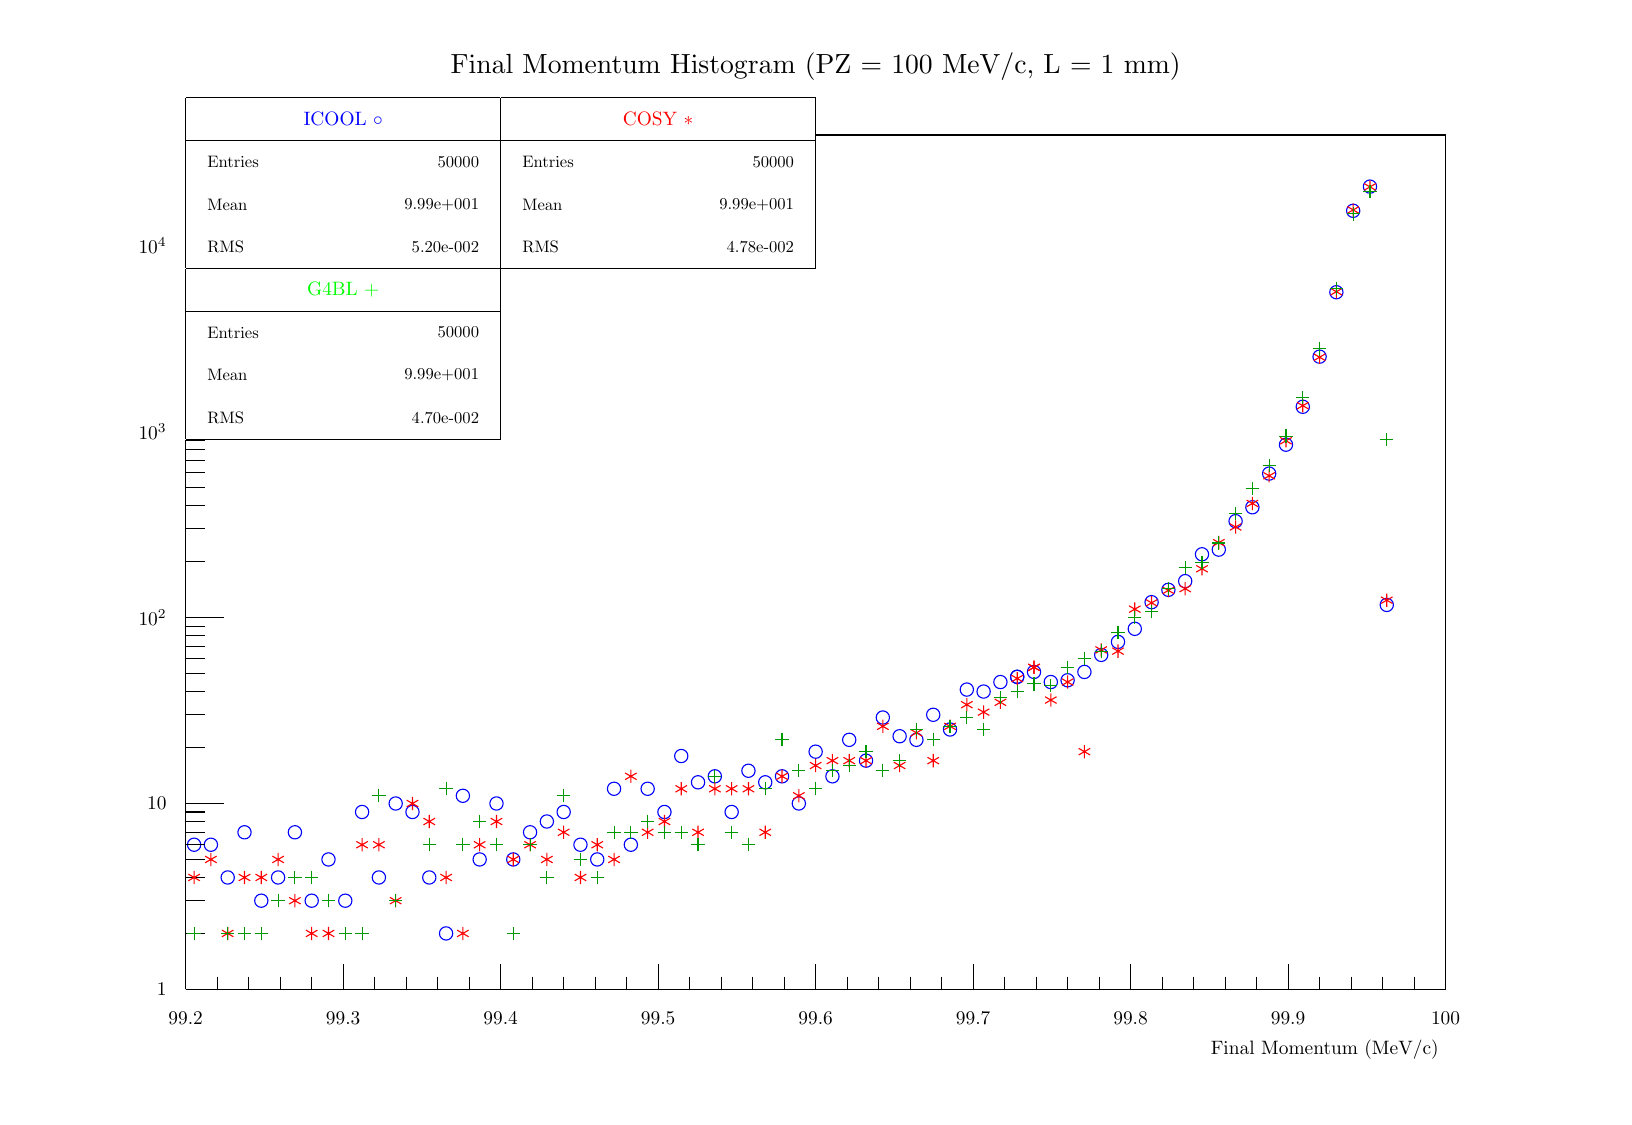
\begin{tikzpicture}
\definecolor{c}{rgb}{1,1,1};
\draw [color=c, fill=c] (0,0) rectangle (20,13.5632);
\draw [color=c, fill=c] (2,1.35632) rectangle (18,12.2069);
\definecolor{c}{rgb}{0,0,0};
\draw [c] (2,1.35632) -- (2,12.2069) -- (18,12.2069) -- (18,1.35632) -- (2,1.35632);
\definecolor{c}{rgb}{1,1,1};
\draw [color=c, fill=c] (2,1.35632) rectangle (18,12.2069);
\definecolor{c}{rgb}{0,0,0};
\draw [c] (2,1.35632) -- (2,12.2069) -- (18,12.2069) -- (18,1.35632) -- (2,1.35632);
\definecolor{c}{rgb}{0,0,1};
\foreach \P in
 {(2.10667,3.19358),(2.32,3.19358),(2.53333,2.77782),(2.74667,3.35164),(2.96,2.48283),(3.17333,2.77782),(3.38667,3.35164),(3.6,2.48283),(3.81333,3.00663),(4.02667,2.48283),(4.24,3.60934),(4.45333,2.77782),(4.66667,3.71737),(4.88,3.60934),(5.09333,2.7
7782),(5.30667,2.06707),(5.52,3.8151),(5.73333,3.00663),(5.94667,3.71737),(6.16,3.00663),(6.37333,3.35164),(6.58667,3.48856),(6.8,3.60934),(7.01333,3.19358),(7.22667,3.00663),(7.44,3.90432),(7.65333,3.19358),(7.86667,3.90432),(8.08,3.60934),(8.29333,
4.32008),(8.50667,3.9864),(8.72,4.06239),(8.93333,3.60934),(9.14667,4.13313),(9.36,3.9864),(9.57333,4.06239),(9.78667,3.71737),(10,4.37552),(10.2133,4.06239),(10.4267,4.52585),(10.64,4.26147),(10.8533,4.80912),(11.0667,4.57143),(11.28,4.52585),(11.49
33,4.84388),(11.7067,4.65693),(11.92,5.16419),(12.1333,5.13887),(12.3467,5.25964),(12.56,5.32582)}{\draw[mark options={color=c,fill=c},mark size=2.402402pt,mark=o] plot coordinates {\P};}
\foreach \P in
 {(12.56,5.32582),(12.7733,5.38798),(12.9867,5.25964),(13.2,5.28218),(13.4133,5.38798),(13.6267,5.60466),(13.84,5.76967),(14.0533,5.93563),(14.2667,6.27388),(14.48,6.43074),(14.6933,6.54095),(14.9067,6.88223),(15.12,6.94136),(15.3333,7.30266),(15.546
7,7.4792),(15.76,7.9071),(15.9733,8.27404),(16.1867,8.75552),(16.4,9.39207),(16.6133,10.2104),(16.8267,11.2444),(17.04,11.5516),(17.2533,6.23941)}{\draw[mark options={color=c,fill=c},mark size=2.402402pt,mark=o] plot coordinates {\P};}
\definecolor{c}{rgb}{1,1,1};
\draw [color=c, fill=c] (2,10.5115) rectangle (6,12.6816);
\definecolor{c}{rgb}{0,0,0};
\draw [c] (2,10.5115) -- (6,10.5115);
\draw [c] (6,10.5115) -- (6,12.6816);
\draw [c] (6,12.6816) -- (2,12.6816);
\draw [c] (2,12.6816) -- (2,10.5115);
\draw[color=blue](4,12.4103) node[scale=0.7, rotate=0]{ICOOL $\circ$};
\draw [c] (2,12.1391) -- (6,12.1391);
\draw [anchor= west] (2.2,11.8678) node[scale=0.6, rotate=0]{Entries };
\draw [anchor= east] (5.8,11.8678) node[scale=0.6, rotate=0]{ 50000};
\draw [anchor= west] (2.2,11.3253) node[scale=0.6, rotate=0]{Mean  };
\draw [anchor= east] (5.8,11.3253) node[scale=0.6, rotate=0]{ 9.99e+001};
\draw [anchor= west] (2.2,10.7828) node[scale=0.6, rotate=0]{RMS   };
\draw [anchor= east] (5.8,10.7828) node[scale=0.6, rotate=0]{ 5.20e-002};
\draw [c] (2,1.35632) -- (18,1.35632);
\draw [anchor= east] (18,0.596782) node[scale=0.7, rotate=0]{Final Momentum (MeV/c)};
\draw [c] (2,1.68184) -- (2,1.35632);
\draw [c] (2.4,1.51908) -- (2.4,1.35632);
\draw [c] (2.8,1.51908) -- (2.8,1.35632);
\draw [c] (3.2,1.51908) -- (3.2,1.35632);
\draw [c] (3.6,1.51908) -- (3.6,1.35632);
\draw [c] (4,1.68184) -- (4,1.35632);
\draw [c] (4.4,1.51908) -- (4.4,1.35632);
\draw [c] (4.8,1.51908) -- (4.8,1.35632);
\draw [c] (5.2,1.51908) -- (5.2,1.35632);
\draw [c] (5.6,1.51908) -- (5.6,1.35632);
\draw [c] (6,1.68184) -- (6,1.35632);
\draw [c] (6.4,1.51908) -- (6.4,1.35632);
\draw [c] (6.8,1.51908) -- (6.8,1.35632);
\draw [c] (7.2,1.51908) -- (7.2,1.35632);
\draw [c] (7.6,1.51908) -- (7.6,1.35632);
\draw [c] (8,1.68184) -- (8,1.35632);
\draw [c] (8.4,1.51908) -- (8.4,1.35632);
\draw [c] (8.8,1.51908) -- (8.8,1.35632);
\draw [c] (9.2,1.51908) -- (9.2,1.35632);
\draw [c] (9.6,1.51908) -- (9.6,1.35632);
\draw [c] (10,1.68184) -- (10,1.35632);
\draw [c] (10.4,1.51908) -- (10.4,1.35632);
\draw [c] (10.8,1.51908) -- (10.8,1.35632);
\draw [c] (11.2,1.51908) -- (11.2,1.35632);
\draw [c] (11.6,1.51908) -- (11.6,1.35632);
\draw [c] (12,1.68184) -- (12,1.35632);
\draw [c] (12.4,1.51908) -- (12.4,1.35632);
\draw [c] (12.8,1.51908) -- (12.8,1.35632);
\draw [c] (13.2,1.51908) -- (13.2,1.35632);
\draw [c] (13.6,1.51908) -- (13.6,1.35632);
\draw [c] (14,1.68184) -- (14,1.35632);
\draw [c] (14.4,1.51908) -- (14.4,1.35632);
\draw [c] (14.8,1.51908) -- (14.8,1.35632);
\draw [c] (15.2,1.51908) -- (15.2,1.35632);
\draw [c] (15.6,1.51908) -- (15.6,1.35632);
\draw [c] (16,1.68184) -- (16,1.35632);
\draw [c] (16.4,1.51908) -- (16.4,1.35632);
\draw [c] (16.8,1.51908) -- (16.8,1.35632);
\draw [c] (17.2,1.51908) -- (17.2,1.35632);
\draw [c] (17.6,1.51908) -- (17.6,1.35632);
\draw [c] (18,1.68184) -- (18,1.35632);
\draw [c] (18,1.68184) -- (18,1.35632);
\draw [anchor=base] (2,0.908736) node[scale=0.7, rotate=0]{99.2};
\draw [anchor=base] (4,0.908736) node[scale=0.7, rotate=0]{99.3};
\draw [anchor=base] (6,0.908736) node[scale=0.7, rotate=0]{99.4};
\draw [anchor=base] (8,0.908736) node[scale=0.7, rotate=0]{99.5};
\draw [anchor=base] (10,0.908736) node[scale=0.7, rotate=0]{99.6};
\draw [anchor=base] (12,0.908736) node[scale=0.7, rotate=0]{99.7};
\draw [anchor=base] (14,0.908736) node[scale=0.7, rotate=0]{99.8};
\draw [anchor=base] (16,0.908736) node[scale=0.7, rotate=0]{99.9};
\draw [anchor=base] (18,0.908736) node[scale=0.7, rotate=0]{100};
\draw [c] (2,1.35632) -- (2,12.2069);
\draw [c] (2.48,1.35632) -- (2,1.35632);
\draw [anchor= east] (1.844,1.35632) node[scale=0.7, rotate=0]{1};
\draw [c] (2.24,2.06707) -- (2,2.06707);
\draw [c] (2.24,2.48283) -- (2,2.48283);
\draw [c] (2.24,2.77782) -- (2,2.77782);
\draw [c] (2.24,3.00663) -- (2,3.00663);
\draw [c] (2.24,3.19358) -- (2,3.19358);
\draw [c] (2.24,3.35164) -- (2,3.35164);
\draw [c] (2.24,3.48857) -- (2,3.48857);
\draw [c] (2.24,3.60934) -- (2,3.60934);
\draw [c] (2.48,3.71737) -- (2,3.71737);
\draw [anchor= east] (1.844,3.71737) node[scale=0.7, rotate=0]{10};
\draw [c] (2.24,4.42812) -- (2,4.42812);
\draw [c] (2.24,4.84388) -- (2,4.84388);
\draw [c] (2.24,5.13887) -- (2,5.13887);
\draw [c] (2.24,5.36768) -- (2,5.36768);
\draw [c] (2.24,5.55463) -- (2,5.55463);
\draw [c] (2.24,5.71269) -- (2,5.71269);
\draw [c] (2.24,5.84962) -- (2,5.84962);
\draw [c] (2.24,5.97039) -- (2,5.97039);
\draw [c] (2.48,6.07843) -- (2,6.07843);
\draw [anchor= east] (1.844,6.07843) node[scale=0.7, rotate=0]{$10^{2}$};
\draw [c] (2.24,6.78917) -- (2,6.78917);
\draw [c] (2.24,7.20493) -- (2,7.20493);
\draw [c] (2.24,7.49992) -- (2,7.49992);
\draw [c] (2.24,7.72873) -- (2,7.72873);
\draw [c] (2.24,7.91568) -- (2,7.91568);
\draw [c] (2.24,8.07374) -- (2,8.07374);
\draw [c] (2.24,8.21067) -- (2,8.21067);
\draw [c] (2.24,8.33144) -- (2,8.33144);
\draw [c] (2.48,8.43948) -- (2,8.43948);
\draw [anchor= east] (1.844,8.43948) node[scale=0.7, rotate=0]{$10^{3}$};
\draw [c] (2.24,9.15022) -- (2,9.15022);
\draw [c] (2.24,9.56598) -- (2,9.56598);
\draw [c] (2.24,9.86097) -- (2,9.86097);
\draw [c] (2.24,10.0898) -- (2,10.0898);
\draw [c] (2.24,10.2767) -- (2,10.2767);
\draw [c] (2.24,10.4348) -- (2,10.4348);
\draw [c] (2.24,10.5717) -- (2,10.5717);
\draw [c] (2.24,10.6925) -- (2,10.6925);
\draw [c] (2.48,10.8005) -- (2,10.8005);
\draw [anchor= east] (1.844,10.8005) node[scale=0.7, rotate=0]{$10^{4}$};
\draw [c] (2.24,11.5113) -- (2,11.5113);
\draw [c] (2.24,11.927) -- (2,11.927);
\definecolor{c}{rgb}{1,1,1};
\draw [color=c, fill=c] (2,10.5115) rectangle (6,12.6816);
\definecolor{c}{rgb}{0,0,0};
\draw [c] (2,10.5115) -- (6,10.5115);
\draw [c] (6,10.5115) -- (6,12.6816);
\draw [c] (6,12.6816) -- (2,12.6816);
\draw [c] (2,12.6816) -- (2,10.5115);
\draw[color=blue](4,12.4103) node[scale=0.7, rotate=0]{ICOOL $\circ$};
\draw [c] (2,12.1391) -- (6,12.1391);
\draw [anchor= west] (2.2,11.8678) node[scale=0.6, rotate=0]{Entries };
\draw [anchor= east] (5.8,11.8678) node[scale=0.6, rotate=0]{ 50000};
\draw [anchor= west] (2.2,11.3253) node[scale=0.6, rotate=0]{Mean  };
\draw [anchor= east] (5.8,11.3253) node[scale=0.6, rotate=0]{ 9.99e+001};
\draw [anchor= west] (2.2,10.7828) node[scale=0.6, rotate=0]{RMS   };
\draw [anchor= east] (5.8,10.7828) node[scale=0.6, rotate=0]{ 5.20e-002};
\draw (10,13.0816) node[scale=1, rotate=0]{Final Momentum Histogram (PZ = 100 MeV/c, L = 1 mm)};
\definecolor{c}{rgb}{1,0,0};
\foreach \P in
 {(2.10667,2.77782),(2.32,3.00663),(2.53333,2.06707),(2.74667,2.77782),(2.96,2.77782),(3.17333,3.00663),(3.38667,2.48283),(3.6,2.06707),(3.81333,2.06707),(4.24,3.19358),(4.45333,3.19358),(4.66667,2.48283),(4.88,3.71737),(5.09333,3.48856),(5.30667,2.7
7782),(5.52,2.06707),(5.73333,3.19358),(5.94667,3.48856),(6.16,3.00663),(6.37333,3.19358),(6.58667,3.00663),(6.8,3.35164),(7.01333,2.77782),(7.22667,3.19358),(7.44,3.00663),(7.65333,4.06239),(7.86667,3.35164),(8.08,3.48856),(8.29333,3.90432),(8.50667
,3.35164),(8.72,3.90432),(8.93333,3.90432),(9.14667,3.90432),(9.36,3.35164),(9.57333,4.06239),(9.78667,3.8151),(10,4.19931),(10.2133,4.26147),(10.4267,4.26147),(10.64,4.26147),(10.8533,4.69715),(11.0667,4.19931),(11.28,4.61507),(11.4933,4.26147),(11.
7067,4.69715),(11.92,4.97222),(12.1333,4.8775),(12.3467,5.00195),(12.56,5.30423),(12.7733,5.44659)}{\draw[mark options={color=c,fill=c},mark size=2.402402pt,mark=asterisk] plot coordinates {\P};}
\foreach \P in
 {(12.7733,5.44659),(12.9867,5.03083),(13.2,5.25964),(13.4133,4.37552),(13.6267,5.66778),(13.84,5.65236),(14.0533,6.18543),(14.2667,6.26538),(14.48,6.42344),(14.6933,6.44518),(14.9067,6.69808),(15.12,7.03021),(15.3333,7.22858),(15.5467,7.52774),(15.7
6,7.87915),(15.9733,8.32343),(16.1867,8.76974),(16.4,9.38476),(16.6133,10.2169),(16.8267,11.2552),(17.04,11.5479),(17.2533,6.299)}{\draw[mark options={color=c,fill=c},mark size=2.402402pt,mark=asterisk] plot coordinates {\P};}
\definecolor{c}{rgb}{1,1,1};
\draw [color=c, fill=c] (6,10.5115) rectangle (10,12.6816);
\definecolor{c}{rgb}{0,0,0};
\draw [c] (6,10.5115) -- (10,10.5115);
\draw [c] (10,10.5115) -- (10,12.6816);
\draw [c] (10,12.6816) -- (6,12.6816);
\draw [c] (6,12.6816) -- (6,10.5115);
\draw [color=red](8,12.4103) node[scale=0.7, rotate=0]{COSY $*$};
\draw [c] (6,12.1391) -- (10,12.1391);
\draw [anchor= west] (6.2,11.8678) node[scale=0.6, rotate=0]{Entries };
\draw [anchor= east] (9.8,11.8678) node[scale=0.6, rotate=0]{ 50000};
\draw [anchor= west] (6.2,11.3253) node[scale=0.6, rotate=0]{Mean  };
\draw [anchor= east] (9.8,11.3253) node[scale=0.6, rotate=0]{ 9.99e+001};
\draw [anchor= west] (6.2,10.7828) node[scale=0.6, rotate=0]{RMS   };
\draw [anchor= east] (9.8,10.7828) node[scale=0.6, rotate=0]{ 4.78e-002};
\definecolor{c}{rgb}{1,1,1};
\draw [color=c, fill=c] (6,10.5115) rectangle (10,12.6816);
\definecolor{c}{rgb}{0,0,0};
\draw [c] (6,10.5115) -- (10,10.5115);
\draw [c] (10,10.5115) -- (10,12.6816);
\draw [c] (10,12.6816) -- (6,12.6816);
\draw [c] (6,12.6816) -- (6,10.5115);
\draw [color=red](8,12.4103) node[scale=0.7, rotate=0]{COSY $*$};
\draw [c] (6,12.1391) -- (10,12.1391);
\draw [anchor= west] (6.2,11.8678) node[scale=0.6, rotate=0]{Entries };
\draw [anchor= east] (9.8,11.8678) node[scale=0.6, rotate=0]{ 50000};
\draw [anchor= west] (6.2,11.3253) node[scale=0.6, rotate=0]{Mean  };
\draw [anchor= east] (9.8,11.3253) node[scale=0.6, rotate=0]{ 9.99e+001};
\draw [anchor= west] (6.2,10.7828) node[scale=0.6, rotate=0]{RMS   };
\draw [anchor= east] (9.8,10.7828) node[scale=0.6, rotate=0]{ 4.78e-002};
\definecolor{c}{rgb}{0,0.6,0};
\foreach \P in
 {(2.10667,2.06707),(2.53333,2.06707),(2.74667,2.06707),(2.96,2.06707),(3.17333,2.48283),(3.38667,2.77782),(3.6,2.77782),(3.81333,2.48283),(4.02667,2.06707),(4.24,2.06707),(4.45333,3.8151),(4.66667,2.48283),(5.09333,3.19358),(5.30667,3.90432),(5.52,3
.19358),(5.73333,3.48856),(5.94667,3.19358),(6.16,2.06707),(6.37333,3.19358),(6.58667,2.77782),(6.8,3.8151),(7.01333,3.00663),(7.22667,2.77782),(7.44,3.35164),(7.65333,3.35164),(7.86667,3.48856),(8.08,3.35164),(8.29333,3.35164),(8.50667,3.19358),(8.7
2,4.06239),(8.93333,3.35164),(9.14667,3.19358),(9.36,3.90432),(9.57333,4.52585),(9.78667,4.13313),(10,3.90432),(10.2133,4.13313),(10.4267,4.19931),(10.64,4.37552),(10.8533,4.13313),(11.0667,4.26147),(11.28,4.65693),(11.4933,4.52585),(11.7067,4.69715)
,(11.92,4.80912),(12.1333,4.65693),(12.3467,5.05893),(12.56,5.13887),(12.7733,5.2366),(12.9867,5.21302)}{\draw[mark options={color=c,fill=c},mark size=2.402402pt,mark=+] plot coordinates {\P};}
\foreach \P in
 {(12.9867,5.21302),(13.2,5.44659),(13.4133,5.55463),(13.6267,5.65236),(13.84,5.88736),(14.0533,6.07842),(14.2667,6.15734),(14.48,6.44518),(14.6933,6.71476),(14.9067,6.77887),(15.12,7.02615),(15.3333,7.40039),(15.5467,7.71427),(15.76,8.00718),(15.973
3,8.38364),(16.1867,8.87017),(16.4,9.49083),(16.6133,10.2611),(16.8267,11.2048),(17.04,11.4935),(17.2533,8.33825)}{\draw[mark options={color=c,fill=c},mark size=2.402402pt,mark=+] plot coordinates {\P};}
\definecolor{c}{rgb}{1,1,1};
\draw [color=c, fill=c] (2,8.34138) rectangle (6,10.5115);
\definecolor{c}{rgb}{0,0,0};
\draw [c] (2,8.34138) -- (6,8.34138);
\draw [c] (6,8.34138) -- (6,10.5115);
\draw [c] (6,10.5115) -- (2,10.5115);
\draw [c] (2,10.5115) -- (2,8.34138);
\draw [color=green](4,10.2402) node[scale=0.7, rotate=0]{G4BL $+$};
\draw [c] (2,9.96897) -- (6,9.96897);
\draw [anchor= west] (2.2,9.6977) node[scale=0.6, rotate=0]{Entries };
\draw [anchor= east] (5.8,9.6977) node[scale=0.6, rotate=0]{ 50000};
\draw [anchor= west] (2.2,9.15517) node[scale=0.6, rotate=0]{Mean  };
\draw [anchor= east] (5.8,9.15517) node[scale=0.6, rotate=0]{ 9.99e+001};
\draw [anchor= west] (2.2,8.61264) node[scale=0.6, rotate=0]{RMS   };
\draw [anchor= east] (5.8,8.61264) node[scale=0.6, rotate=0]{ 4.70e-002};
\definecolor{c}{rgb}{1,1,1};
\draw [color=c, fill=c] (2,8.34138) rectangle (6,10.5115);
\definecolor{c}{rgb}{0,0,0};
\draw [c] (2,8.34138) -- (6,8.34138);
\draw [c] (6,8.34138) -- (6,10.5115);
\draw [c] (6,10.5115) -- (2,10.5115);
\draw [c] (2,10.5115) -- (2,8.34138);
\draw [color=green](4,10.2402) node[scale=0.7, rotate=0]{G4BL $+$};
\draw [c] (2,9.96897) -- (6,9.96897);
\draw [anchor= west] (2.2,9.6977) node[scale=0.6, rotate=0]{Entries };
\draw [anchor= east] (5.8,9.6977) node[scale=0.6, rotate=0]{ 50000};
\draw [anchor= west] (2.2,9.15517) node[scale=0.6, rotate=0]{Mean  };
\draw [anchor= east] (5.8,9.15517) node[scale=0.6, rotate=0]{ 9.99e+001};
\draw [anchor= west] (2.2,8.61264) node[scale=0.6, rotate=0]{RMS   };
\draw [anchor= east] (5.8,8.61264) node[scale=0.6, rotate=0]{ 4.70e-002};
\end{tikzpicture}
